%%%%%%%%%%%%%%%%%%%%%%%%%%%%%%%%%%%%%%%%%
% a0poster Portrait Poster
% LaTeX Template
% Version 1.0 (22/06/13)
%
% The a0poster class was created by:
% Gerlinde Kettl and Matthias Weiser (tex@kettl.de)
% 
% This template has been downloaded from:
% http://www.LaTeXTemplates.com
%
% License:
% CC BY-NC-SA 3.0 (http://creativecommons.org/licenses/by-nc-sa/3.0/)
%
%%%%%%%%%%%%%%%%%%%%%%%%%%%%%%%%%%%%%%%%%

%----------------------------------------------------------------------------------------
%	PACKAGES AND OTHER DOCUMENT CONFIGURATIONS
%----------------------------------------------------------------------------------------

\documentclass[a0,portrait]{a0poster}

\usepackage{multicol} % This is so we can have multiple columns of text side-by-side
\columnsep=75pt % This is the amount of white space between the columns in the poster
\columnseprule=1pt % This is the thickness of the black line between the columns in the poster

\usepackage[svgnames]{xcolor} % Specify colors by their 'svgnames', for a full list of all colors available see here: http://www.latextemplates.com/svgnames-colors

\usepackage{times} % Use the times font
%\usepackage{palatino} % Uncomment to use the Palatino font

\usepackage{graphicx} % Required for including images
\graphicspath{{figures/}} % Location of the graphics files
\usepackage{booktabs} % Top and bottom rules for table
\usepackage[font=small,labelfont=bf]{caption} % Required for specifying captions to tables and figures
\usepackage{amsfonts, amsmath, amsthm, amssymb} % For math fonts, symbols and environments
\usepackage{wrapfig} % Allows wrapping text around tables and figures
\usepackage{tabularx}
\begin{document}

%----------------------------------------------------------------------------------------
%	POSTER HEADER 
%----------------------------------------------------------------------------------------

% The header is divided into two boxes:
% The first is 75% wide and houses the title, subtitle, names, university/organization and contact information
% The second is 25% wide and houses a logo for your university/organization or a photo of you
% The widths of these boxes can be easily edited to accommodate your content as you see fit

\begin{minipage}[b]{0.75\linewidth}
\veryHuge \color{NavyBlue} \textbf{Are Online Users with Us ? Deep Representation Learning for Political Stance Detection} \color{Black}\\ % Title
\Huge\textit{5th International Conference on Computational Social Science}\\[0.5cm]% Subtitle
\huge \textbf{Zoya Khan, Priyam Bansal Mansi Sharma, Rishabh Kaushal}\\ % Author(s)
\huge Indira Gandhi Delhi Technical University for Women, New Delhi, India\\ % University/organization

\end{minipage}
%
\begin{minipage}[b]{0.25\linewidth}

\includegraphics[width=10cm]{igdtuw_logo.jpg}\\

\includegraphics[width=10cm]{ic2s2.png}\\
\end{minipage}

\vspace{0.5cm} % A bit of extra whitespace between the header and poster content

%----------------------------------------------------------------------------------------

\begin{multicols}{2} % This is how many columns your poster will be broken into, a portrait poster is generally split into 2 columns

%----------------------------------------------------------------------------------------
%	ABSTRACT
%----------------------------------------------------------------------------------------

\color{Navy} % Navy color for the abstract

\begin{abstract}

Stance detection is the task of estimating a user's opinion about a particular issue, whether the user is `towards', `against' or `neutral' to the topic. In this study, we aim to predict the political stance of a user by using a sophisticated, state of the art Deep Learning autoencoder model. This is the first study that focuses on the complex Indian political scenario, where there are multiple political parties catering to the diverse populace. Our model takes a textual statement (tweet) as input and follows a two step classification for detecting stance. A first level classifier identifies whether the text is stance revealing or not. Only stance revealing tweets are then fed as input to the second level classifier which aims to correctly identify the political allegiance of the user on a six-point scale of being Pro or Anti of the three major political parties that influence the politics of Delhi, namely Aam Aadmi Party (AAP), Bharatiya Janata Party (BJP), and the Indian National Congress (INC). When compared with traditional models like word2vec and Google Pre-trained embeddings for learning word embeddings, our autoecoder based model performs strikingly better.
Our implementation of the autoencoder is a sequence to sequence model having LSTM based Encoder and Decoder models. The intermediate output of the autoencoder is fed to multiple classification algorithms, with Random Forest giving best accuracy.
\end{abstract}

%----------------------------------------------------------------------------------------
%	INTRODUCTION
%----------------------------------------------------------------------------------------

\color{SaddleBrown} % SaddleBrown color for the introduction

\section*{Introduction}

With the advent of social media, online social networking sites like Twitter, Facebook, Reddit, Instagram, etc have become popular platforms for political discussions and debates. This expression of political views creates an opportunity for both politicians and citizens, with the former benefiting two-fold, firstly by being able to better understand the opinions of the people and secondly to be able to effectively disseminate political information in a targeted manner.
\textit{Stance detection is the task of detecting a user’s opinion. It aims at understanding the sentiment of a given text and understanding if it is in favour (positive), is against (negative) or is neutral towards a given proposition or target. This target may be a person, an organization, a government policy, a movement, a product, etc.}
In this study we aim at detecting the political stance of users living in and around the National Capital of Territory (NCT) of Delhi, India. We focus our interest on three major political parties like the Aam Aadmi Party (AAP), Bhartiya Janata Party (BJP) and the Indian National Congress (INC) that have played a crucial role in shaping the political scenario of Delhi and are hence the primary centre of our interest.
Unlike bi-partisan democracies like the USA, India's polity is much more complex owing to the prevalence of many political parties catering to the diversities in India. This is the first study that focuses on the complex Indian political scenario, where there are numerous national as well as regional political parties.

%----------------------------------------------------------------------------------------
%	RELATED WORKS
%----------------------------------------------------------------------------------------

\color{DarkSlateGray} % DarkSlateGray color for the rest of the content

% \section*{Related Works}.
% In early studies, various linguistic features are used to predict the stance using data from congressional debates\cite{thomas2006get} and online debates on public forums \cite{somasundaran2009recognizing}\cite{walker2012stance}. With the development of Online Social Media networks, stance detection on tweets has become popular. Unlike debates, which contain automatically annotated data, annotated tweets for stance detection are limited, hence, unsupervised or semi-supervised methods for detecting stance on tweets come up - like a weakly supervised approach to detect stance held by politicians proposed by Johnson et. al\cite{johnson2016identifying}, an LSTM based attention model for topical stance detection proposed by Dey et. al\cite{dey2018topical} and retweet-based label propagation algorithm proposed by Addawod et. al\cite{addawood2017stance}.\\
% SemEval task 6\cite{mohammad2016semeval} is a groundbreaking work in this domain where numerous techniques are proposed, best result being MITRE \cite{zarrella2016mitre} where word2vec skip gram model\cite{mikolov2013efficient} is used to create word embeddings and then those features are used to learn sentence representations via a hashtag prediction auxiliary task. We use an autoencoder for creating word embeddings, which proves to be better than word2vec approach. Dey et. al\cite{dey2018topical} use SemEval data and detected topical stance using a two phase technique as proposed in this study; where an LSTM based deep neural network is used for for each phase, and embed attention at each of the phases. In this study, we use Indian tweets and use an autoencoder to create word embeddings and detect stance of tweets in two phases.
%----------------------------------------------------------------------------------------
%	DATA
%----------------------------------------------------------------------------------------

\section*{Data}
\subsection*{Identification of Twitter Users and Tweet Collection}
We collect tweets related to political parties in the national capital region of Delhi in India, the largest democracy in the world, focusing on three parties namely, Aam Aadmi Party (AAP), Bhartiya Janta Party (BJP) and the Indian National Congress (INC).
We search for the target users by using Twitter's Advanced Search to search for tweets which contain certain hashtags like - \#BJP, \#AAP, \#INC, \#politics, \#elections  etc. to identify users who actively tweet about politics. 
We then manually analyze the tweets on each user's profile to determine which political party they support or are against and label each user in the following categories:\\ \textit{Pro AAP, Pro BJP, Pro INC, Anti AAP, Anti BJP, Anti INC, Neutral}\\
A total of 245 users were identified by conducting this search. For this study we do not consider Twitter accounts of verified profiles, political party leaders, popular politicians, media \& news profiles and also of users residing outside Delhi. We collect the Twitter timelines of all these users with a language filter that allows only "English Language" tweets of the users to be stored in the database. At the end of this phase we have 3,76,932 tweets with us stored in the database.
In order to concentrate our focus only on tweets with some politic context, we create a natural language based political filter to extract only politically relevant tweets from the 3,76,932 tweet corpus that we have. To create this filter we begin by creating a comprehensive dictionary of keywords that are usually used in the context of Indian Politics. This filter reduces these 3,76,932 tweets into 1,53,032 tweets.
\subsection*{Manual Annotation Of Tweets}
To create ground truth, we manually annotate tweets at two levels. 
\begin{itemize}
    \item At \textit{first level}, we provide a binary label (0 or 1) depending upon whether the tweet is stance neutral or stance revealing.
    \item At \textit{second level}, we give six labels from 1 to 6, indicating Pro-AAP, Pro-BJP, Pro-INC, Anti-AAP, Anti-BJP \& Anti-INC, respectively.
\end{itemize} 
We select a subset of political tweets to annotate manually by randomly selecting 50 political tweets from each user and get 10,932 tweets at the end of this phase. All the tweets are shuffled and then given to the annotator. The annotations were done by strictly abiding to a set of annotation guidelines which were formulated for this purpose.
\begin{center}\vspace{1cm}
\begin{tabular}{l p{35cm} }
\toprule
1 & Only the tweet text is taken into consideration for the annotation process and the annotator is not given access to any detail of the tweeter.\\
2 & Any URLs present in the tweet text have to be ignored by the annotator.\\
3 & Tweets addressing only AAP, BJP and/or INC are to be annotated. If a tweet addresses any other political party besides these three, it is labelled 0. However, if a tweet has a mention of any other political party, but also consists of a mention of AAP, BJP and/or INC, it will be annotated.\\ 
4 & If a tweet indicates the speaker's political preference or allegiance, it is labelled 1.\\
5 & If a tweet indicates that the speaker is against a political party, it is labelled 1.\\ 
6 & If a tweet is a general political statement and does not reveal anything about his/her support or criticism of any party, it is labelled 0.\\
7 & A tweet with personal comments on a politician is labelled 0.\\
8 & If a tweet praises or criticizes a government reform or policy and does not comment about any party, it is labelled 0.\\
\bottomrule
\end{tabular}
\captionof{table}{\color{Green} Guidelines for Label 1 annotation}
\end{center}

% \begin{center}\vspace{1cm}
% \begin{tabular}{p{30cm}| l} 
% \toprule
% \textbf{Tweet Text} & \textbf{Label} \\
% \midrule
%  "Why don’t you put the unedited tapes online @republic? If it was anyone with money, there’d be a defamation case against the \#FakeNews outfit. Republic TV is dumbing our nation down and causing radicalisation. I say this even though the channel is pro \#BJP. https://t.co/J73cXNfnCy" & 1 \\ 
% \midrule
%  "This happened when u elect DUMB \#OurPMissoDUMB" & 1 \\  
% \midrule
%  "@TimesNow Shashi Tharoor knows his wife's murder case is closing \&amp; his role in the murder will be exposed- This is a tested evil strategy- Go make anti-Hindu, communal and anti-India comments and when he is convicted and jailed he will claim political vendetta" & 0 \\
% \midrule
%   "@AmaninderZ @sprakaashbjp @DeShobhaa Politics was never clean not because of politicians, coz they are one of us.. Its their wickd thoughts" & 0 \\ 
% \midrule
%  "@thekiranbedi People like you are needed in national politics. We bank on you!" & 0 \\  
% \midrule

%  "\#Demonetisation did cause distress but was a huge one-time shock to the black money economy Alongwith \#GST (the biggest systemic reform since 1947), lasting impact on formalising economy Still not sure? Just check status of cash-based business models eg. real estate, pvt edu etc https://t.co/DYz0EmPLem" & 0 \\  
% \bottomrule
% \end{tabular}
% \captionof{table}{\color{Green} Some Examples of Label 1 annotation}
% \end{center}
\begin{center}\vspace{1cm}
\begin{tabular}{l p{35cm} }
\toprule
1 & Only tweets with Label 1 as '1' are to be annotated.\\
2 & Labelling of one tweet for both the labels should be done in one pass by the annotator.\\
3 & If a tweet is favouring, praising or showing support to Aam Aadmi Party (AAP) it is labelled 1.\\
4 & If a tweet is favouring, praising or showing support to Bhartiya Janata Party (BJP) it is labelled 2.\\
5 & If a tweet is favouring, praising or showing support to Indian National Congress (INC) it is labelled 3.\\
6 & If a tweet is criticizing or trolling Aam Aadmi Party (AAP) it is labelled 4.\\
7 & If a tweet is criticizing or trolling Bhartiya Janata Party (BJP) it is labelled 5.\\
8 & If a tweet is criticizing or trolling Indian National Congress (INC) it is labelled 6.\\
9 & If a tweet fits a pro category (1,2 or 3) as well as an anti category (4,5 or 6), it is marked with the pro category label i.e either 1,2 or 3.\\ 
10 & If a tweet fits in more than one pro category labels it is not annotated and its Label 1 value is changed to 0.\\
11 & If a tweet fits in more than one anti category and none of the pro categories, it is not annotated and its Label 1 value is changed to 0.\\
12 & If a tweet fits in more than one anti category and also in one pro category, it is given the pro label i.e 1,2 or 3.\\
\bottomrule
\end{tabular}
\captionof{table}{\color{Green} Guidelines for Label 2 annotation}
\end{center}

% \begin{center}\vspace{1cm}
% \begin{tabular}{p{30cm}| l} 
% \toprule
% \textbf{Tweet Text} & \textbf{Label} \\
% \midrule
% "New DELHI GOVT. School\'s building. We need SCHOOLS not TEMPLES. We need Educated not Brainwashed Uneducated INDIA. We need Educated Honest Leaders not Uneducated Corrupted Criminals \#AAP \#AAPGoverment \#DelhiGoverment \#ArvindKejriwal \#ManishSisodia... https://t.co/jRqNnScZP5" & 1 \\ 
% \midrule
% "Save this. Frame this. Narendra Modi\'s historic \#AbkiBaarModiSarkaar win heralded on countless front pages. http://t.co/ZX9xF0gj7B" & 2 \\  
% \midrule
% "\@Mnomics \@rockyindian7 \@AAPVind \@alamgirizvi \@jayambadi \@logicalindianz \@BreakiNews \@RafaleScam \@SkepticHindu \@DickDarryl \@KilaFateh \@INCIndia They don’t have any heritage any history, whatever RSS has is full of blood; hatred, so it’s very easy to make fun of someone whose entire lineage has laid down their lives for this country." & 3 \\
% \midrule
% "\#KejriDiwas AAP ditched the people of Delhi by bringing down its Government to take the plunge in the national political arena" & 4 \\
% \midrule
% "The \#BJP \&amp; \@IASassociation have colluded to sabotage the image the \@ArvindKejriwal/\#AAP Govt has built over the years. They have total disregard 4 democratically elected representatives. \#Modi ji, dont punish the Delhiites bcz they chose Kejriwal over u. \@attorneybharti https://t.co/3qVpYD5LQ0" & 5 \\
% \midrule
% "\@Goldiepandey26 \@GetRidofDevils Absolutely true. Its established fact. Basic problem is that \#RahulGandhi is in illusion that he is prince of \#NehruGandhi dynasty n has birth right to rule India.His sycophants never tell him that India is under democracy and he is nothing more than comedian." & 6 \\
% \bottomrule
% \end{tabular}
% \captionof{table}{\color{Green} Some Examples of Label 2 annotation}
% \end{center}
%----------------------------------------------------------------------------------------
%	RESULTS 
%----------------------------------------------------------------------------------------

\section*{Methodology}
We propose a deep learning model that follows an approach of using an LSTM based autoencoder to create tweet-level vectors that capture the context of the tweet. It then performs a two level classification using these intermediate vectors to first detect stance revealing tweets and then further detect the stance of these tweets.

\begin{center}\vspace{1cm}
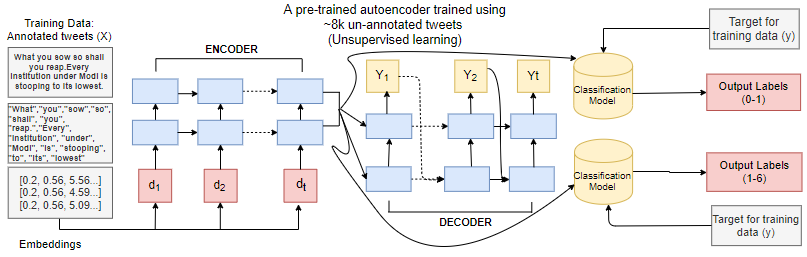
\includegraphics[width=0.8\linewidth]{autoencoder.png}
\captionof{figure}{\color{Green} Autoencoder}
\end{center}\vspace{1cm}

An autoencoder is an unsupervised deep learning algorithm that attempts to reconstruct the input that was fed to it by creating an intermediate representation of the input. The autoencoder then attempts to reconstruct the initial input given this intermediate representation. The following equations govern the functioning of the autoencoder:
\begin{equation}
     \omega: A \to B (Encoder)
 \end{equation}
 \begin{equation}
     \gamma: B \to A (Decoder)
 \end{equation}

We contextualize the autoencoder as a sequence to sequence model containing Recurrent Neural Network based Encoder and Decoder models. We then feed these embeddings to classification algorithms like Random Forest, Decision Tree, Naive Bayes and Support Vector Machine and compare their performance on two levels i.e. classification of a tweet into stance-revealing or not and another classification model to detect the stance of the tweet.

\section*{Results}

We compare with autoencoder based approach with two baselines.
\begin{enumerate}
    \item Word2vec (w2v) Model \cite{mikolov2013efficient}: It is a neural network based model, trained on the vocabulary of the input dataset to generate word vectors. To represent phrase (tweet) level vectors, we take the mean of word vectors as suggested by Mikolov et. al. \cite{mikolov2013distributed}. 
    \item Google Embedding: It is Google's Pre-trained word embeddings created by Mikolov et. al. \cite{mikolov2013distributed} and trained on the Google news data. 
\end{enumerate}

\begin{center}\vspace{1cm}
\begin{tabular}{l l l l} 
\toprule
\textbf{Model} & \textbf{word2vec} & \textbf{Google's Pre-trained} & \textbf{Autoencoder}\\
\midrule
Naive Bayes & 0.481 & 0.641 & 0.155 \\ 
Random Forest & 0.774 & 0.759 & 0.849 \\  
Decision Tree & 0.643  & 0.657 & 0.799 \\
Support Vector Classifier & 0.774  & 0.759 & 0.849 \\
\bottomrule
\end{tabular}
\captionof{table}{\color{Green} Scores for all classification models after phase 1}
\end{center}
%----------------------------------------------------------------------------------------
%	CONCLUSIONS
%----------------------------------------------------------------------------------------

\color{SaddleBrown} % SaddleBrown color for the conclusions to make them stand out

\section*{Conclusions}

The results show that the autoencoder gives the highest efficiency as compared to word2vec and google pre-trained word embeddings on our dataset. The autoencoder's performance can be attributed to the efficient representation of the input that it creates, it is hence able to better predict the stance from the tweet. Google's Pre-trained word embeddings also prove to be a good option to serve as default embeddings as it achieves good baseline results.

\color{DarkSlateGray} % Set the color back to DarkSlateGray for the rest of the content

%----------------------------------------------------------------------------------------
%	FORTHCOMING RESEARCH
%----------------------------------------------------------------------------------------


 %----------------------------------------------------------------------------------------
%	REFERENCES
%----------------------------------------------------------------------------------------

\bibliographystyle{plain} % Plain referencing style
\bibliography{sample} % Use the example bibliography file sample.bib

\end{multicols}
\end{document}